% Embed2Heights — architecture diagram (clean orthogonal layout)
% Compile:  tectonic architecture.tex   ->  architecture.pdf
\documentclass[border=12pt]{standalone}
\usepackage[T1]{fontenc}
\usepackage{tikz}
\usepackage{amsmath}
\usetikzlibrary{positioning,arrows.meta,fit,backgrounds,calc}

\definecolor{cAlpha}{HTML}{1b6ca8}   % dense pixel embeddings
\definecolor{cToken}{HTML}{c8553d}   % coarse token embeddings
\definecolor{cHead} {HTML}{2a7f62}   % heads / tasks
\definecolor{cOut}  {HTML}{6a4c93}   % outputs
\definecolor{cGray} {HTML}{555555}

\begin{document}
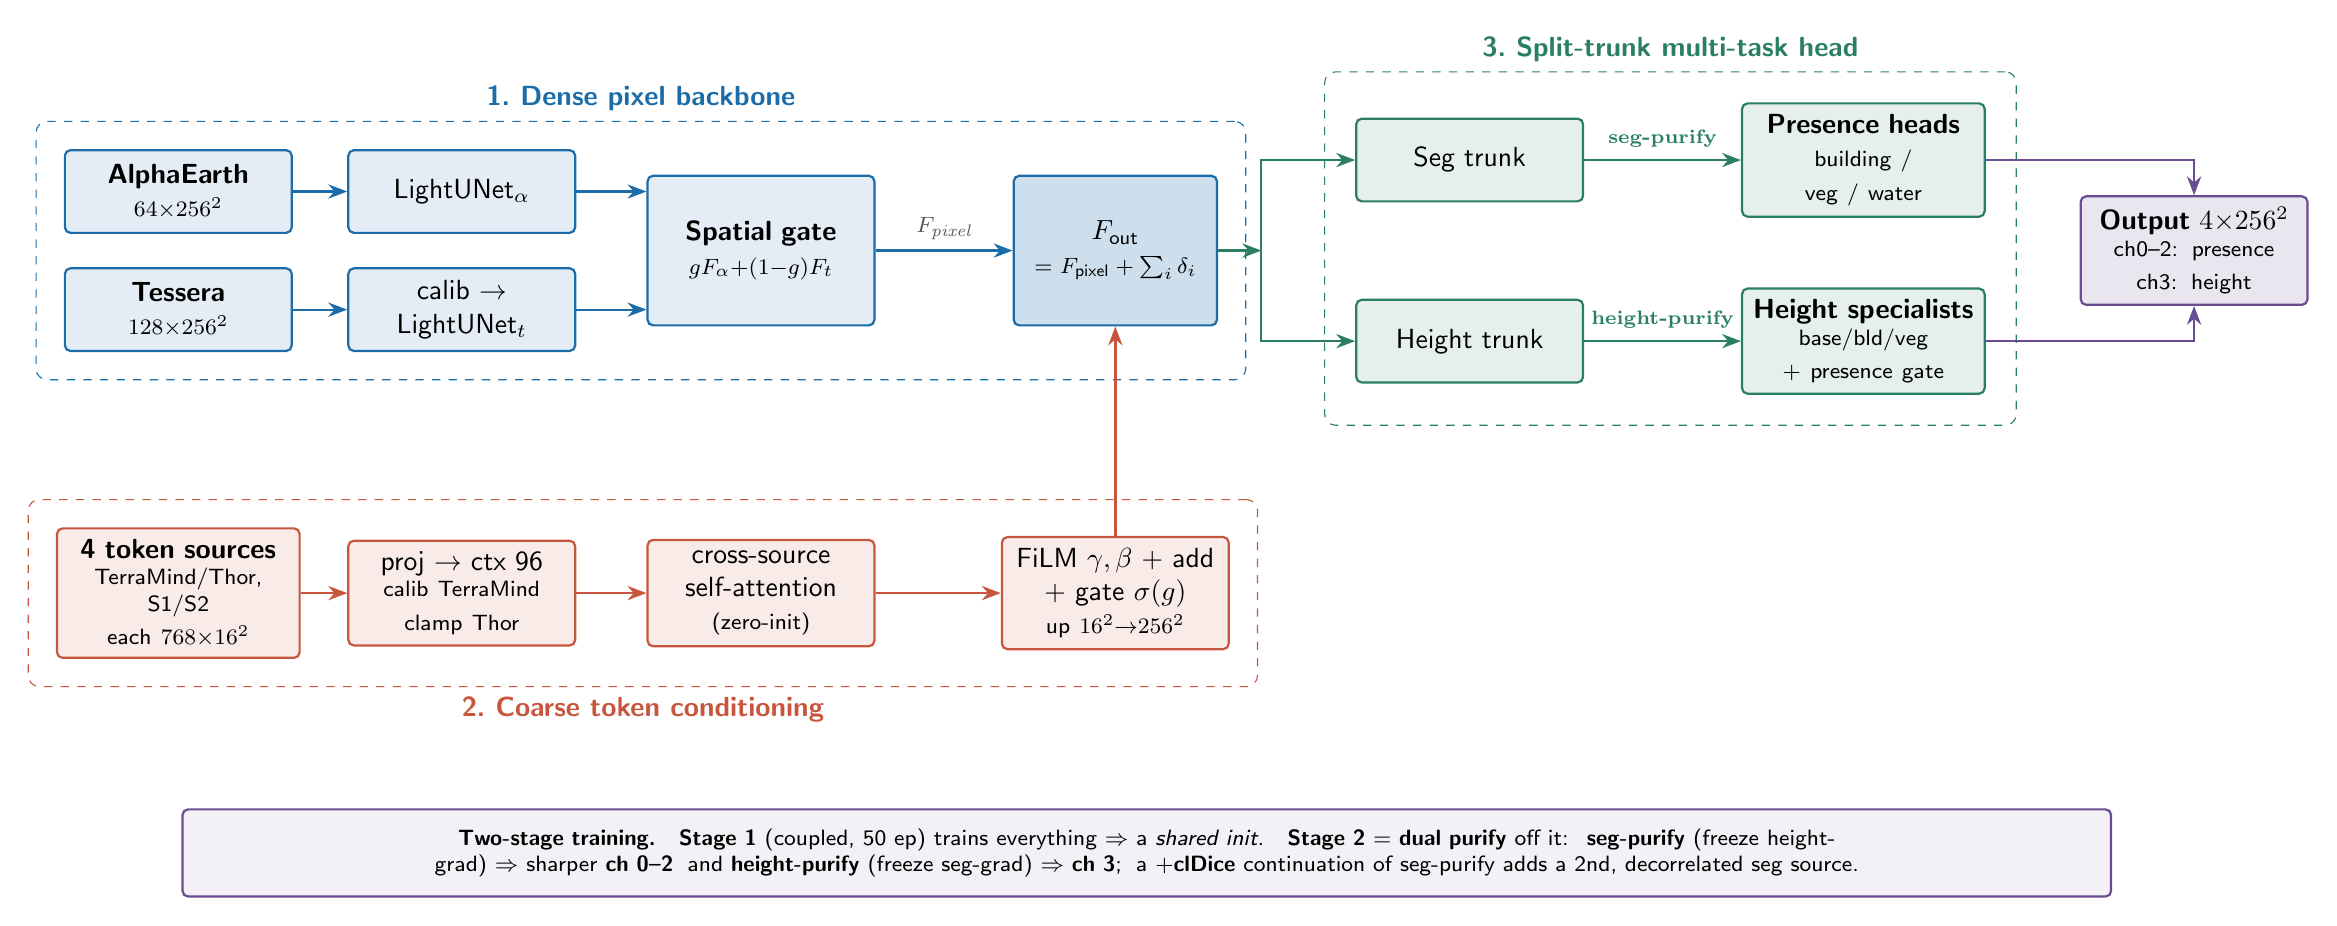
\begin{tikzpicture}[
    x=1cm,y=1cm,font=\sffamily,
    >={Stealth[length=2.4mm]},
    box/.style={rounded corners=2pt,draw,thick,align=center,inner sep=4pt,
                minimum height=1.05cm,text width=2.6cm},
    pix/.style={box,fill=cAlpha!12,draw=cAlpha},
    tok/.style={box,fill=cToken!12,draw=cToken},
    hd/.style ={box,fill=cHead!12,draw=cHead},
    op/.style ={box,fill=cOut!14,draw=cOut},
    fp/.style ={box,fill=cAlpha!22,draw=cAlpha,text width=2.3cm},
    ar/.style ={->,thick},
    arp/.style={->,thick,cAlpha},
    art/.style={->,thick,cToken},
    arh/.style={->,thick,cHead},
    aro/.style={->,thick,cOut},
    capt/.style={font=\footnotesize\itshape,cGray},
    tag/.style ={font=\scriptsize\bfseries},
  ]

  % ---------- PIXEL BAND (top) ----------
  \node[pix] (ae)   at (0,3.0)  {\textbf{AlphaEarth}\\\footnotesize $64{\times}256^2$};
  \node[pix] (tes)  at (0,1.5)  {\textbf{Tessera}\\\footnotesize $128{\times}256^2$};
  \node[pix] (aenc) at (3.6,3.0){LightUNet$_\alpha$};
  \node[pix] (tenc) at (3.6,1.5){calib $\to$ LightUNet$_t$};
  \node[pix,minimum height=1.9cm] (gate) at (7.4,2.25)
        {\textbf{Spatial gate}\\\footnotesize $g F_\alpha{+}(1{-}g)F_t$};
  \node[fp,minimum height=1.9cm] (fp) at (11.9,2.25)
        {$F_{\text{out}}$\\\footnotesize $=F_{\text{pixel}}+\sum_i\delta_i$};

  \draw[arp] (ae) -- (aenc);
  \draw[arp] (tes) -- (tenc);
  \draw[arp] (aenc.east) -- (gate.west|-aenc.east);
  \draw[arp] (tenc.east) -- (gate.west|-tenc.east);
  \draw[arp,line width=1pt] (gate) -- (fp) node[midway,above,capt]{$F_{\text{pixel}}$};

  % ---------- TOKEN BAND (bottom) ----------
  \node[tok,text width=2.8cm] (toks) at (0,-2.1)
        {\textbf{4 token sources}\\\footnotesize TerraMind/Thor, S1/S2\\\footnotesize each $768{\times}16^2$};
  \node[tok] (proj) at (3.6,-2.1)
        {proj $\to$ ctx 96\\\footnotesize calib TerraMind\\\footnotesize clamp Thor};
  \node[tok] (attn) at (7.4,-2.1)
        {cross-source\\self-attention\\\footnotesize (zero-init)};
  \node[tok] (inj) at (11.9,-2.1)
        {FiLM $\gamma,\beta$ + add\\+ gate $\sigma(g)$\\\footnotesize up $16^2{\to}256^2$};

  \draw[art] (toks) -- (proj);
  \draw[art] (proj) -- (attn);
  \draw[art] (attn) -- (inj);
  \draw[art,line width=1pt] (inj) -- (fp);   % single clean vertical merge

  % ---------- HEAD (split-trunk) ----------
  \node[hd] (segt) at (16.4,3.4) {Seg trunk};
  \node[hd] (hgtt) at (16.4,1.1) {Height trunk};
  \node[hd,text width=2.8cm] (sheads) at (21.4,3.4)
        {\textbf{Presence heads}\\\footnotesize building / veg / water};
  \node[hd,text width=2.8cm] (hspec) at (21.4,1.1)
        {\textbf{Height specialists}\\\footnotesize base/bld/veg\\\footnotesize + presence gate};

  % clean T-split out of F_out
  \coordinate (sp) at ($(fp.east)+(0.55,0)$);
  \draw[arh,line width=1pt] (fp.east) -- (sp);
  \draw[arh] (sp) |- (segt.west);
  \draw[arh] (sp) |- (hgtt.west);
  % stage-2 dual-purify tags on the two trunk branches
  \draw[arh] (segt) -- (sheads) node[midway,above=1pt,tag,cHead]{seg-purify};
  \draw[arh] (hgtt) -- (hspec) node[midway,above=1pt,tag,cHead]{height-purify};

  % ---------- OUTPUT ----------
  \node[op,text width=2.6cm] (out) at (25.6,2.25)
        {\textbf{Output} $4{\times}256^2$\\\footnotesize ch0--2: presence\\\footnotesize ch3: height};
  \draw[aro] (sheads.east) -| (out.north);
  \draw[aro] (hspec.east)  -| (out.south);

  % ---------- GROUPING BOXES ----------
  \begin{scope}[on background layer]
    \node[draw=cAlpha,dashed,rounded corners,inner sep=10pt,fit=(ae)(tenc)(gate)(fp),
          label={[cAlpha,font=\sffamily\bfseries]above:1.\ Dense pixel backbone}] {};
    \node[draw=cToken,dashed,rounded corners,inner sep=10pt,fit=(toks)(inj),
          label={[cToken,font=\sffamily\bfseries]below:2.\ Coarse token conditioning}] {};
    \node[draw=cHead,dashed,rounded corners,inner sep=11pt,fit=(segt)(hgtt)(sheads)(hspec),
          label={[cHead,font=\sffamily\bfseries]above:3.\ Split-trunk multi-task head}] {};
  \end{scope}

  % ---------- TWO-STAGE (DUAL-PURIFY) CAPTION ----------
  \node[op,fill=cOut!8,draw=cOut,text width=24cm,align=center,inner sep=7pt,
        font=\sffamily\footnotesize] at (12.3,-5.4) {%
     \textbf{Two-stage training.}\quad
     \textbf{Stage 1} (coupled, 50 ep) trains everything $\Rightarrow$ a \emph{shared init}.\quad
     \textbf{Stage 2 $=$ dual purify} off it:\;
     \textbf{seg-purify} (freeze height-grad) $\Rightarrow$ sharper \textbf{ch 0--2}\;
     and \textbf{height-purify} (freeze seg-grad) $\Rightarrow$ \textbf{ch 3};\;
     a \textbf{$+$clDice} continuation of seg-purify adds a 2nd, decorrelated seg source.};

\end{tikzpicture}
\end{document}
